\chapter{Other Tools}

	
	\section{\texttt{wavespec}: Spectral analysis tools}

	Some spectral analysis tools for analyzing waves in data.
	
	\subsection{Installation}
	
	\subsubsection{Using \texttt{pip3}:}
	
	\begin{minted}{bash}
	pip3 install wavespec --user
	\end{minted}
	
	\subsubsection{Installing the wheel using \texttt{pip3}:}
	
	\begin{minted}{bash}
	pip3 install wavespec-0.0.1-py3-none-any.whl --user
	\end{minted}
	
	\subsubsection{From git:}
	 
	\begin{minted}{bash}
	git clone https://github.com/mattkjames7/wavespec
	cd wavespec
	python3 setup.py install --user
	\end{minted}
	
	\subsection{Usage}
	
	\begin{minted}{python}
	import wavespec as ws
	\end{minted}
	
	\subsubsection{Fast Fourier Transform (FFT)}
	
	\begin{minted}{python}
	power,phase,freq,fr,fi = ws.Fourier.FFT(t,x,WindowFunction=None,Param=None)
	\end{minted}
	
	\subsubsection{Lomb-Scargle (LS)}
	
	\begin{minted}{python}
	P,A,phi,a,b = ws.LombScargle.LombScargle(t,x0,f,Backend='C++',WindowFunction=None,Param=None)
	\end{minted}
	
	\subsubsection{Spectrograms}
	
	\begin{minted}{python}
	Nw,LenW,Freq,out = ws.Spectrogram.Spectrogram(t,v,wind,slip,Freq=None,Method='FFT',WindowFunction=None,Param=None,Detrend=True,FindGaps=True,GoodData=None,Quiet=True,LenW=None)
	
	ax,Nw,LenW,Freq,Spec = ws.Spectrogram.PlotSpectrogram(t,v,wind,slip,Freq=None,Method='FFT',WindowFunction=None,Param=None,Detrend=True,FindGaps=True,GoodData=None,Quiet=True,LenW=None,fig=None,maps=[1,1,0,0],PlotType='Pow',scale=None,zlog=False,TimeAxisUnits='s',FreqAxisUnits='Hz')
	\end{minted}
	
	\subsubsection{3D Spectrograms}
	
	\begin{minted}{python}
	Nw,LenW,Freq,Spec = ws.Spectrogram.Spectrogram3D(t,vx,vy,vz,wind,slip,Freq=None,Method='FFT',WindowFunction=None,Param=None,Detrend=True,FindGaps=False,GoodData=None)
	\end{minted}
	
	\subsubsection{Tests}
	
	\begin{minted}{python}
	ws.Test.TestLS(A=[1.0,2.0],f=[0.04,0.1],phi=[0.0,90.0],Backend='C++')
	ws.Test.TestPolarization(xPow=2.0,xPhase=0.0,yPow=1.0,yPhase=40.0)
	ws.Test.TestSpectrogram()
	\end{minted}
	

	\section{\texttt{MHDWaveHarmonics}: Tools for MHD waves}
	
	Some simple tools for modelling MHD wave harmonics in an arbitrary magnetic field geometry.
	
	\subsection{Installation}
	
	Install using \texttt{pip3}:
	
	\begin{minted}{bash}
	pip3 install MHDWaveHarmonics --user
	\end{minted}
	
	The installation will require the following packages:
	
	\begin{itemize}
	  \item \texttt{numpy}
	  \item \texttt{scipy}
	  \item \texttt{matplotlib}
	  \item \texttt{PyGeopack}
	  \item \texttt{FieldTracing}
	\end{itemize}
	
	all of which will be installed automatically. For modelling waves in
	Mercury's magnetosphere, you will also require the \texttt{KT17} model.
	
	\subsection{Usage}
	
	\subsubsection{1. \texttt{GetFieldLine}}
	
	The \texttt{GetFieldLine} function will trace a model field, returning a 
	\texttt{TraceField} object alongside a \texttt{numpy.ndarray}, \texttt{s}, which contains the 
	distance along the traced field line and optionally \texttt{h} if the 
	polarization is specified:
	
	\begin{minted}{python}
	import MHDWaveHarmonics as wh
	T,s = wh.GetFieldLine(pos,Date=None,ut=None,Model='KT17',Delta=None,Polarization='none',**kwargs)
	T,s,h = wh.GetFieldLine(pos,Date=None,ut=None,Model='KT17',Delta=None,Polarization='poloidal',**kwargs)
	\end{minted}
	
	where \texttt{h} is provided using a second trace if the \texttt{Polarization} parameter
	is set to \texttt{'poloidal'}, \texttt{'toroidal'}, or a \texttt{float} corresponding to an
	angle in degrees anticlockwise from the poloidal direction (the outward
	pointing normal direction of the field line). Use \texttt{wh.GetFieldLine?}
	to find out more about this procedure from its docstring.
	
	\subsubsection{2. \texttt{SolveWave}}
	
	This procedure will attempt to solve the wave equation along an arbitrary
	magnetic field trace such as that provided by \texttt{GetFieldLine}:
	
	\begin{minted}{python}
	yr = wh.SolveWave(f,x,B,R=None,Va=None,halpha=None,Params=None,InPlanet=None,Method='Simple',Unscale=True)
	yr,yi,phase = SolveWave(f,x,B,R=None,Va=None,halpha=None,Params=None,InPlanet=None,Method='Complex',Unscale=True)
	\end{minted}
	
	where \texttt{yr} is the real part of the scaled field displacement, $\xi/h_\alpha$, \texttt{yi} 
	is the imaginary part, and \texttt{phase} is a continuous measure of the waves
	phase along the trace. See the docstring for more information.
	
	\subsubsection{3. \texttt{FindHarmonics}}
	
	This will attempt to solve the wave equation to find a number
	of harmonics that would be allowed to exist:
	
	\begin{minted}{python}
	freq,success,niter = wh.FindHarmonics(T,s,Params,halpha=None,Harmonics=[1,2,3],x0=None,df=1.0,Method='Complex')
	\end{minted}
	
	where \texttt{freq} is an array of allowed frequencies, \texttt{success} is a Boolean 
	array denoting whether each fit was successful or not, and \texttt{niter} is an 
	array containing the number of iterations required for each fit.
	
	\subsubsection{4. \texttt{CalcFieldLineVa}}
	
	This will calculate the Alfven speed at each point along the trace:
	
	\begin{minted}{python}
	va = CalcFieldLineVa(T,s,Params,halpha=None)
	\end{minted}
	
	or at the midpoint between each pair of consecutive steps along the trace:
	
	\begin{minted}{python}
	vamid = CalcFieldLineVaMid(T,s,Params,halpha=None)
	\end{minted}
	
	\subsubsection{5. \texttt{PlotHarmonics}}
	
	This will produce a plot of the allowed toroidal and poloidal harmonics 
	on a field line given an initial position for the trace and a plasma
	mass density profile along the field.
	
	\begin{minted}{python}
	PlotHarmonics(pos,Params,nh=3,df=1.0,Rp=1.0,Colours=None,Method='Complex',**kwargs)
	\end{minted}
	
	\subsubsection{6. \texttt{FitPlasmaToHarmonic}}
	
	Attempts to fit a power law or the Sandhu et al model plasma mass density
	profile to a given field trace.
	
	\begin{minted}{python}
	p_eq = FitPlasmaToHarmonic(T,s,halpha,f,Params,Harm=1,df=1.0,Method='Complex')
	\end{minted}
	
	\subsubsection{7. \texttt{FitPlasma}}
	
	This tries to fit the plasma mass density profile to a set of observed
	frequencies (with their assumed harmonic numbers) along a field trace.
	
	\begin{minted}{python}
	params = FitPlasma(T,s,halpha,freqs,harms,Params0,df=1.0,Method='Complex',ParamFit=None)
	\end{minted}
	
	\subsubsection{8. \texttt{GetSandhuParams}}
	
	Calculates the parameters for the Sandhu et al electron density and 
	average ion mass models.
	
	\begin{minted}{python}
	ne0,alpha,a,beta,mav0 = GetSandhuParams(mlt,L)
	\end{minted}
	
	\subsubsection{9. \texttt{PlotFieldLineDensity}}
	
	Plots the modelled density along a field line given a position in which
	to start a field trace and a set of plasma profile parameters.
	
	\begin{minted}{python}
	PlotFieldLineDensity(pos,Params,fig=None,maps=[1,1,0,0],Overplot=False,**kwargs)
	\end{minted}
	
	
	
	\section{\texttt{FieldTracing}: Python field tracing code}
	

	This is a very simple Python module to trace fields (e.g., magnetic fields) when provided with a model.
	
	\subsection{Installation}
	
	Install using \texttt{pip3}:
	
	\begin{minted}{bash}
	pip3 install --user FieldTracing
	\end{minted}
	
	Or by cloning this repo:
	
	\begin{minted}{bash}
	#clone the repo
	git clone https://github.com/mattkjames7/FieldTracing
	cd FieldTracing
	
	#Either create a wheel and use pip: (X.X.X should be replaced with the current version)
	python3 setup.py bdist_wheel
	pip3 install --user dists/FieldTracing-X.X.X-py3-none-any.whl
	
	#Or by using setup.py directly
	python3 setup.py install --user
	\end{minted}
	
	\subsection{Usage}
	
	There are two tracing routines in this model: \texttt{FieldTracing.Euler.EulerTrace} - this is the most basic tracing routine, which will step in the direction of the field using the Euler method; \texttt{FieldTracing.RK4.RK4Trace} - this uses the 4th order Runge-Kutta method. If you are tracing any non-linear field, the \texttt{RK4} method would most likely be the better choice.
	
	For more information about keywords and arguments supplied to each function:
	
	\begin{minted}{python}
	import FieldTracing as ft
	
	ft.RK4.RK4Trace?
	ft.Euler.EulerTrace?
	\end{minted}
	
	Below is an example trace using the \texttt{KT17} model field module (see \url{https://github.com/mattkjames7/KT17}):
	
	\begin{minted}{python}
	import KT17
	import FieldTracing as ft
	import matplotlib.pyplot as plt
	
	#define a model field function which will accept a vector position and return a field vector
	def modelfunc(p):
		#accepts position with shape (3,)
		B = KT17.ModelField(p[0],p[1],p[2])
		#return field with shape (3,)
		return np.array(B).flatten()
	
	#define a function which says whether we are within some acceptable tracing bounds
	def boundsfunc(p):
		#check if we are within the planet (note that Mercury has a vertical dipole offset)
		r = np.sqrt(p[0]**2 + p[1]**2 + (p[2]+0.196)**2)
		#we want this to terminate at the surface of the iron core, so we should return True as long as r > 0.83
		return r > 0.83
	
	#call the field tracing function, from some initial position
	x0 = [1.2,0.0,0.0]
	Tr = ft.RK4.RK4Trace(x0,0.02,modelfunc,bounds=boundsfunc)
	Te = ft.Euler.EulerTrace(x0,0.02,modelfunc,bounds=boundsfunc)
	
	#call the built-in KT17 trace
	T = KT17.TraceField(*x0,LimType=17)
	
	#plot to compare
	a = np.arange(361)*np.pi/180.0
	x = np.cos(a)
	z = np.sin(a) - 0.196
	xc = 0.83*np.cos(a)
	zc = 0.83*np.sin(a) - 0.196
	plt.figure()
	ax = plt.subplot2grid((1,1),(0,0))
	ax.plot(x,z,color=[0.0,0.0,0.0,0.7],label='Mercury Surface',lw=4)
	ax.plot(xc,zc,color=[0.5,0.5,0.5,0.7],label='Mercury Core',linestyle='--',lw=4)
	ax.plot(Tr[:,0],Tr[:,2],color='red',label='FieldTrace (RK4)')
	ax.plot(Te[:,0],Te[:,2],color='lime',label='FieldTrace (Euler)')
	ax.plot(T.x,T.z,color='blue',label='KT17.TraceField',linestyle=':')
	ax.set_xlabel('$x_{MSM}$')
	ax.set_ylabel('$z_{MSM}$')
	ax.set_aspect(1.0)
	ax.legend()
	\end{minted}
	
	Which should produce this:
	
	\begin{figure}[H]
		\centering
		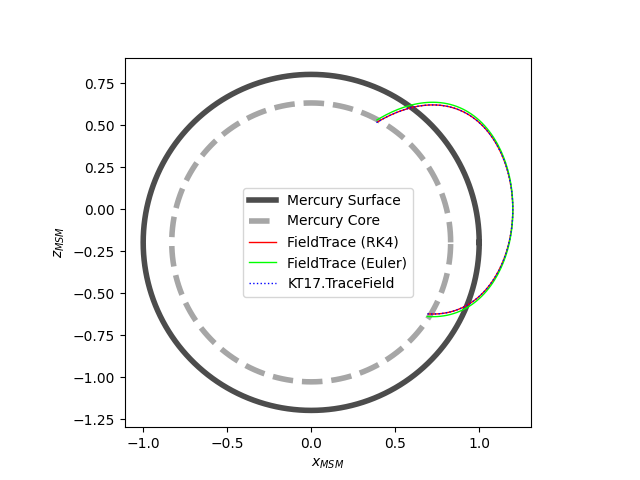
\includegraphics[width=0.7\textwidth]{figures/ch7_ftExample.png}
		\caption{Example trace}
	\end{figure}
	
	
	\section{\texttt{DateTimeTools}: Tools for dealing with dates and times}


A package containing some simple tools to manage dates and times.

\subsection{Installation}

Install using \texttt{pip3}:

\begin{minted}{bash}
pip3 install DateTimeTools --user
\end{minted}

NOTE: This module uses a C++ backend, which is compiled with \texttt{g++} under Linux (libdatetime.so) and Windows 10 (libdatetime.dll). This code has mostly been tested in Linux (Mint 20ish, CentOS 7) with a very brief test in Windows 10. The precompiled libraries may fail to load under other versions of both operating systems (definitely on Mac, or 32-bit OSes) - if so, then the module will attempt to recompile itself on the host system using \texttt{g++}. If recompilation fails, please check that you have \texttt{g++} installed - under Linux install GCC, under Windows install Mingw GCC (I used TDM-GCC, be sure to select \texttt{g++}).

\subsection{Usage}

\subsubsection{Converting between different date/time formats}

Usually this package deals with integer dates in the format \texttt{yyyymmdd} and floating point times in hours since the start of the day.

We can convert to a few different time formats:

\begin{minted}{python}
import DateTimeTools as TT

Date = 20140102
ut = 15.0

#to unix time (seconds since 00:00 1970-01-01)
unixt = TT.UnixTime(Date,ut)
#and back
Date,ut = TT.UnixTimetoDate(unixt)

#to continuous time (hours since 00:00 1950-01-01)
utc = TT.ContUT(Date,ut)
#and back again
Date,ut = TT.contUTtoDate(utc)

#Julian day
jd = TT.JulDay(Date,ut)
#and back
Date,ut = TT.JulDaytoDate(jd)

#CDF Epoch (milliseconds since 00:00 0000-01-01)
cdfe = TT.CDFEpoch(Date,ut)
#and back
Date,ut = TT.CDFEpochtoDate(cdfe)

#get the python datetime
dt = TT.Datetime(Date,ut)
#or the reverse conversion
Date,ut = TT.DatetimetoDate(dt)

#convert hours since the start of the day to hours,minutes,seconds,milliseconds
hh,mm,ss,ms = TT.DectoHHMM(ut)
#and back
ut = TT.HHMMtoDec(hh,mm,ss,ms)

#Split dates into separate integers
yr,mn,dy = TT.DateSplit(Date)
#or the reverse
Date = TT.DateJoin(yr,mn,dy)
\end{minted}

\subsubsection{Formatted plot tick marks}

The \texttt{DTPlotLabel} function can be used to change the plot labels on the x-axis of a \texttt{matplotlib.pyplot} plot such that they resemble human-readable times and dates.

For example:

\begin{minted}{python}
import matplotlib.pyplot as plt

#some plot of a time series
#t is time either in unix time, ContUT, seconds from the start of the day
#or hours from the start of the day
plt.plot(t,x) 
ax = plt.gca()

#if we are plotting with t = TT.ContUT(Date,ut) 
#the function will be able to work out the date
#The TimeFMT keyword isn't needed here, by default = 'utc'
TT.DTPlotLabel(ax)

#similar to above - we can us unix time
#so t = TT.UnixTime(Date,ut)
#We must let the function know though
TT.DTPlotLabel(ax,TimeFMT='unix')

#With seconds from the beginning of the day, we need to
#tell the function what Date starts at t == 0.0
#NOTE t can go beyond the range 0 < t < 24,
#the labels should include relevant dates
#Also, without the date keyword, just HH:MM(:SS) is shown
TT.DTPlotLabel(ax,TimeFMT='seconds',Date=20150101)

#Plotting with hours since the start of the day is similar
TT.DTPlotLabel(ax,TimeFMT='hours',Date=20190908)
\end{minted}

\subsubsection{Calculating time differences}

\begin{minted}{python}
#calculate the difference between two dates in days
ndays = TT.DateDifference(Date0,Date1)

#Similar to above, but include start and end times (still returns days)
ndays = TT.TimeDifference(Date0,ut0,Date1,ut1)

#We can find the middle time between two date/times
mDate,mut = TT.MidTime(Date0,ut0,Date1,ut1)
\end{minted}

\subsubsection{Filtering time series data}

Given an evenly sampled time series, the \texttt{lsfilter} function can perform low-pass and high-pass filtering.

\begin{minted}{python}
#t is the evenly sampled time axis
#x is the time series data

#we need to know the sampling interval in seconds
inter = t[1] - t[0]

#we can do a low-pass filter, we need to set 'high = inter'
#and 'low = lsec' which is the cutoff period in seconds
xlow = TT.lsfilter(x,inter,lowsec,inter)

#alternatively a high-pass filter can be used by setting
#'high = hsec' (the cutoff period in seconds) and 'low = inter'
xhigh = TT.lsfilter(x,hsec,inter,inter)
\end{minted}

\subsubsection{Miscellaneous functions}

\begin{minted}{python}
#calculate day number and year
year,dayno = TT.DayNo(Date)
#or return to original date format
Date = TT.DayNotoDate(year,dayno)

#Check if year(s) are leap year(s)
ly = TT.LeapYear(year)

#Add one day to a date
NextDate = TT.PlusDay(Date)
#or go back a day
PrevDate = TT.MinusDay(Date)

#Calculate the nearest index in a time/date array
#to a test time/date
ind = TT.NearestTimeIndex(DateArray,utArray,testDate,testut)

#check which indices of a time array are within two time limits
inds = TT.WithinTimeRange(t,t0,t1)
#or including dates
inds = TT.WithinTimeRange((d,t),(d0,t0),(d1,t1))
%alternatively, return a boolean array where each True element is within the range
b = TT.WithinTimeRange((d,t),(d0,t0),(d1,t1),BoolOut=True)
\end{minted}



	\section{\texttt{datetime}: C++ library dealing for dates and times}


	A C++ library containing some time-related tools.
	
	\subsection{Installation}
	
	This library requires GNU-make and g++ to be built in Linux and Mac. In Windows, I use TDM-GCC to provide the C++ compiler.
	
	Clone the repo:
	
	\begin{minted}{bash}
	git clone https://github.com/mattkjames7/datetime.git
	cd datetime
	\end{minted}
	
	For Linux or Mac:
	\begin{minted}{bash}
	#build the library
	make
	
	#optionally install globally
	sudo make install
	\end{minted}
	
	For Windows:
	\begin{minted}{cmd}
	> compile.bat
	\end{minted}
	
	\subsection{Linking}
	
	To link to this library in C or C++, you should include the header for the library:
	
	\begin{minted}{cpp}
	#include <datetime.h>
	\end{minted}
	
	then link to the library, e.g.:
	
	\begin{minted}{bash}
	#when installed globally
	g++ $(CFLAGS) main.cc -o main -ldatetime
	
	#otherwise
	g++ $(CFLAGS) -I/path/to/header/ main.cc -o main -L/path/to/lib -ldatetime
	\end{minted}
	
	\subsection{Testing}
	
	To check that all of the functions are working as expected, run the following tests in Linux/Mac:
	
	\begin{minted}{bash}
	make test
	\end{minted}
	
	or in Windows:
	
	\begin{minted}{cmd}
	> test.bat
	\end{minted}
	
	If the library has been installed globally, then the following test will check that linking can be done to the globally installed lib/header:
	
	\begin{minted}{bash}
	make testinstall
	\end{minted}
	
	\subsection{Summary of Functions}
	
	\begin{tabular}{|l|l|}
	\hline
	Name & Description \\
	\hline
	\href{include/datetime.h#L34}{\mintinline{text}{ContUT()}} & Converts Date and UT to a continuous value of hours since 19500101 00:00. \\
	\href{include/datetime.h#L51}{\mintinline{text}{ContUTtoDate()}} & Converts output of \mintinline{text}{ContUT()} back to date and time. \\
	\href{include/datetime.h#L69}{\mintinline{text}{DateDifference()}} & Find the number of days between two dates. \\
	\href{include/datetime.h#L87}{\mintinline{text}{DateJoin()}} & Join the individual elements of a date (year, month and day) to a single integer with the format \_yyyymmdd. \\
	\href{include/datetime.h#L105}{\mintinline{text}{DateSplit()}} & Split the date integer into year, month, and day. \\
	\href{include/datetime.h#L123}{\mintinline{text}{DayNo()}} & Converts a date of the format \_yyyymmdd to year and day number. \\
	\href{include/datetime.h#L140}{\mintinline{text}{DayNotoDate()}} & Converts year and day number to a date with the format \_yyyymmdd. \\
	\href{include/datetime.h#L159}{\mintinline{text}{DectoHHMM()}} & Converts the time in decimal hours to hours, minutes, seconds, and milliseconds. \\
	\href{include/datetime.h#L177}{\mintinline{text}{HHMMtoDec()}} & Converts hours, minutes, seconds, and milliseconds to decimal hours. \\
	\href{include/datetime.h#L193}{\mintinline{text}{JulDay()}} & Converts a date and time to Julian day. \\
	\href{include/datetime.h#L209}{\mintinline{text}{JulDaytoDate()}} & Converts Julian day to date and time. \\
	\href{include/datetime.h#L224}{\mintinline{text}{LeapYear()}} & Determines whether a year is a leap year or not. \\
	\href{include/datetime.h#L242}{\mintinline{text}{MidTime()}} & Works out the time and date exactly in the middle of two dates/times. \\
	\href{include/datetime.h#L257}{\mintinline{text}{MinusDay()}} & Subtracts one day from a date. \\
	\href{include/datetime.h#L277}{\mintinline{text}{NearestTimeIndex()}} & Finds the index of a time array closest to a given date/time. \\
	\href{include/datetime.h#L292}{\mintinline{text}{PlusDay()}} & Adds a day to a date. \\
	\href{include/datetime.h#L310}{\mintinline{text}{TimeDifference()}} & Calculates the time difference (in days) between two dates/times. \\
	\href{include/datetime.h#L329}{\mintinline{text}{UnixTime()}} & Calculate the Unix time given a date and time. \\
	\href{include/datetime.h#L346}{\mintinline{text}{UnixTimetoDate()}} & Convert Unix time back to date and UT. \\
	\href{include/datetime.h#L369}{\mintinline{text}{WithinTimeRange()}} & Find the indices of a time array that lie within two dates/times. \\
	\hline
	\end{tabular}
	

	\section{\texttt{PyFileIO}: Tools for reading and writing files}


	Some very basic routines for file IO in Python
	
	\subsection{Installation}
	
	Install via \mintinline{text}{pip3}:
	
	\begin{minted}{bash}
	pip3 install PyFileIO --user
	\end{minted}
	
	or from this repo:
	
	\begin{minted}{bash}
	git clone https://github.com/mattkjames7/PyFileIO
	cd PyFileIO
	
	#either this
	python3 setup.py install --user
	
	#or this
	python3 setup.py bdist_wheel
	pip3 install dist/PyFileIO-X.X.X-py3-none-any.whl
	\end{minted}
	
	where \mintinline{text}{X.X.X} is the version created.
	
	\subsection{Usage}
	
	This module contains a few different methods of loading/saving data.
	
	\subsubsection{Loading/Saving Objects}
	
	This effectively uses \mintinline{text}{pickle} to load and save physical objects, e.g.:
	
	\begin{minted}{python}
	import PyFileIO as pf
	
	#save an object
	pf.SaveObject(obj,'/path/to/some/file.bin')
	
	#load an object
	obj = pf.LoadObject('/path/to/some/file.bin')
	\end{minted}
	
	\subsubsection{Loading/Saving ASCII Data}
	
	Text files may be created and read directly:
	
	\begin{minted}{python}
	#saving text
	text = 'some text, can be an array\n or just a single string'
	pf.WriteASCIIFile('filename.txt',text)
	
	#reading text
	text = pf.ReadASCIIFile('filename.txt')
	\end{minted}
	
	We can also use ASCII files to load \mintinline{text}{csv} files and save data stored in a simple \mintinline{text}{numpy.recarray}:
	
	\begin{minted}{python}
	#read a csv file, which contains a header - dtype will be worked out automatically
	data = pf.ReadASCIIData('somedata.csv')
	
	#we can also save data
	pf.WriteASCIIData('newfile.dat',data)
	\end{minted}
	
	NOTE: this will only work with simple \mintinline{text}{dtypes}
	
	\subsubsection{Loading/Saving Binary Data}
	
	Pure binary data may be written to files using the following functions:
	
	\begin{minted}{python}
	#open a file
	f = open('filename.bin','wb')
	
	#save some stuff
	ScalarToFile(x,'int64',f)       #save a single scalar integer
	ArrayToFile(y,'float32',f)      #save a floating point array
	ListArrayToFile(z,'int32',f)    #save a list of integer arrays
	StringToFile(s,f)               #save a string to file
	
	#close the file
	f.close()
	\end{minted}
	
	We can also read the data back (remembering to use the correct dtypes!):
	
	\begin{minted}{python}
	#open a file
	f = open('filename.bin','rb')
	
	#read the stored data
	x = ScalarFromFile('int64',f)       #read a single scalar integer
	y = ArrayFromFile('float32',f)      #read a floating point array
	z = ListArrayFromFile('int32',f)    #read a list of integer arrays
	s = StringFromFile(f)               #read a string from file
	
	#close the file
	f.close()
	\end{minted}
	

	\section{\texttt{RecarrayTools}: Tools for manipulating \texttt{numpy.recarrays}}	


	Some simple tools for managing \mintinline{python}{numpy.recarray} objects
	
	\subsection{Installation}
	
	Install via \mintinline{text}{pip}:
	
	\begin{minted}{bash}
	pip3 install --user RecarrayTools
	\end{minted}
	
	Or this repo:
	
	\begin{minted}{bash}
	#clone the repo
	git clone https://github.com/mattkjames7/RecarrayTools
	cd RecarrayTools
	
	#either use a wheel
	python3 setup.py bdist_wheel
	pip3 install --user dist/RecarrayTools-0.0.3-py3-none-any.whl
	
	#or just install directly
	python3 setup.py install
	\end{minted}
	
	\subsection{Usage}
	
	This module contains a small number of routines...
	
	\subsubsection{\texttt{SaveRecarray()}}
	
	This will save a record array to a binary file - note that the dtype of the record array shouldn't be too exotic (object arrays would not work - use pickle for those).
	
	\begin{minted}{python}
	import numpy as np
	import RecarrayTools as RT
	
	#create some recarray
	dtype = [('a','int32'),('b','float64',(6,))]
	arr = np.recarray(10,dtype=dtype)
	
	#fill it
	arr.a = blah #shape (10,)
	arr.b = stuff #shape (10,6)
	
	#save it
	RT.SaveRecarray(arr,'path/to/file.name',Progress=True)
	\end{minted}
	
	The file format used here is simple:
	
	The first 4 bytes correspond to a 32-bit integer containing the size of the recarray (i.e. \mintinline{python}{arr.size}).
	
	Then each field \mintinline{python}{arr.dtype.names} is stored contiguously as whatever dtype it was assigned with, one field at a time.
	
	The file created in the above example would be formatted in the following way:
	
	Bytes 0-3: 32-bit integer - total length of the recarray
	
	Bytes 4-43: Array of 32-bit integers, length 10 (\mintinline{python}{arr.a})
	
	Bytes 44-523: Array of 64-bit floating points, shape (10,6), length 60
	
	EOF
	
	\subsubsection{\texttt{ReadRecarray()}}
	
	This will read in the files created by \texttt{SaveRecarray()}, e.g.
	
	\begin{minted}{python}
	dtype = [('a','int32'),('b','float64',(6,))]
	fname = 'path/to/file.name'
	arr = RT.ReadRecarray(fname,dtype)
	\end{minted}
	
	\subsubsection{\texttt{ReduceRecarray()}}
	
	This reduces the number of fields in a recarray object, e.g.:
	
	\begin{minted}{python}
	#initial object with fields 'a', 'b', 'c' and 'd'
	dtype = [('a','int32'),('b','float64',(6,)),('c','int64'),('d','float64')]
	obj0 = np.recarray(10,dtype=dtype)
	
	#new object with just fields 'a' and 'c'
	obj1 = RT.ReduceRecarray(obj0,['a','c'])
	\end{minted}
	
	\subsubsection{\texttt{JoinRecarray()}}
	
	Append two recarrays with identical dtypes:
	
	\begin{minted}{python}
	C = RT.JoinRecarray(A,B)
	\end{minted}
	
	\subsubsection{\texttt{AppendFields()}}
	
	Append some extra fields to a recarray:
	
	\begin{minted}{python}
	#some initial recarray
	A = np.recarray(n,dtype=dtype)
	
	#new fields for the array
	x = np.arange(n)
	y = x**2
	
	#add them
	B = RT.AppendFields(A,[('x','float32'),('y','float32')],(x,y))
	#B now has fields B.x and B.y
	\end{minted}
	
	\subsubsection{\texttt{InterpRecarrayFields()}}
	
	Interpolate fields within a recarray:
	
	\begin{minted}{python}
	#a would be the initial recarray, b would be the new recarray
	#RefField = name of field to interpolate over
	#InterpFields = list of names of fields to interpolate
	b = RT.InterpRecarrayFields(a,b,RefField='x',InterpFields=['a','b','c','d','x'])
	\end{minted}
	

	\section{\texttt{PBSJobExamples}: Examples for submitting jobs to ALICE}


	TL;DR: Copy one of these folders, \mintinline{text}{$cd} into it, add your python code to "runcode.py", edit myjob.sub to have the correct vram etc., then run \mintinline{text}{$ ./submitjob.sh}
	
	\subsection{Templates}
	
	This folder contains three templates: "singlejob", "arrayjob" and "paralleljob". Each contains four files which can be tweaked as necessary and one output folder ("out/") which \texttt{stdout} and \texttt{stderr} are written to while the job is running.
	
	\subsubsection{singlejob}
	
	This template can be used to submit a single job.
	
	\subsubsection{arrayjob}
	
	This tamplate can be used to submit an array of jobs, where, for example, the same bit of code may be run in each instance, but on a different set of parameters (e.g. date).
	
	The relevant part of the job submission code:
	
	\begin{minted}{bash}
	#PBS -t 1-1000
	\end{minted}
	
	where \texttt{1-1000} indicates a range of job indices from 1 to 1000. This could also be an explicit list, e.g. \texttt{2,5,7,99}.
	
	\subsubsection{paralleljob}
	
	This is an example of a parallelised job. This is also an array job, but it is also applicable to single jobs. This will run code which, in each instance, will use multiple cores (e.g. using openMP) and/or nodes (e.g. using openMPI).
	
	The relevant part of the job submission script:
	
	\begin{minted}{bash}
	#PBS -l nodes=1:ppn=8
	\end{minted}
	
	where \texttt{nodes=1} denotes the number of nodes over which this code can be distributed upon, and \texttt{ppn=8} states how many processors to assign per node.
	
	\subsection{Job Files}
	
	It is important that "submitjob.sh" and "startscript.sh" are marked as executable, e.g.
	
	\begin{minted}{bash}
	chmod +x submitjob.sh
	\end{minted}
	
	\subsubsection{submitjob.sh}
	
	This script will submit the job to the cluster by running the command: \mintinline{text}{$ ./submitjob.sh} 
	
	While it isn't necessary -  it pretty much just calls the \texttt{qsub} command, it saves some typing and it passes the current working directory to the job script so that the correct output folder is used.
	
	\subsubsection{myjob.sub}
	
	This contains all of the job configuration options, e.g.
	
	\begin{minted}{bash}
	#PBS -v WD
	\end{minted}
	
	This passes environment variables from the current session (where the job is submitted) to the running code. In this case \texttt{WD} is the working directory provided in "submitjob.sh".
	
	\begin{minted}{bash}
	#PBS -o out/output.txt
	\end{minted}
	
	This is the name of the output file where \texttt{stdout} will be saved.
	
	\begin{minted}{bash}
	#PBS -e out/error.txt
	\end{minted}
	
	This is the output error file where \texttt{stderr} will be saved.
	
	\begin{minted}{bash}
	#PBS -N ParallelArrayJob
	\end{minted}
	
	This is the name of the job.
	
	\begin{minted}{bash}
	#PBS -l walltime=0:15:00
	\end{minted}
	
	This is the total amount of time for the job to run in \texttt{hh:mm:ss}. For longer jobs, add days before hours, e.g. \texttt{dd:hh:mm:ss}.
	
	\begin{minted}{bash}
	#PBS -l vmem=20gb
	\end{minted}
	
	This is the total amount of virtual memory to assign to the job. Ideally, this should not be much more than what it actually requires (more jobs can run at a time in that case).
	
	\begin{minted}{bash}
	#PBS -m bea
	\end{minted}
	
	This tells the cluster to send an email when each job begins \texttt{b}, ends \texttt{e} or is aborted \texttt{a}. Be warned - this will send those emails for each element of an array job!
	
	\begin{minted}{bash}
	#PBS -l nodes=1:ppn=8
	\end{minted}
	
	This is for jobs which will be able to use more than one single thread. \texttt{nodes} is the number of nodes requested for each instance of the job. \texttt{ppn} is the number of processors to assign for each node.
	
	\begin{minted}{bash}
	#PBS -t 1-50
	\end{minted}
	
	Array job range.
	
	After the \texttt{\#PBS} options are defined, the rest of this file can be treated as a \texttt{bash} script which will be executed when the job starts. In this case, each job will call \mintinline{text}{$WD/startscript.sh} - this isn't necessary, the commands from within "startscript.sh" can be placed directly within this job submission file if desired.
	
	\subsubsection{startscript.sh}
	
	This file contains the commands to be called when each job runs. It can be placed directly in "myjob.sub", but a separate script is used here. This file is where \texttt{python} or \texttt{idl} may be called, for example.
	
	\subsubsection{runcode.py}
	
	This file contains the python code to run in the job. It assumes that the job to be submitted will be running \texttt{python} and can be replaced with scripts for other languages as needed.
	
	For array jobs, it is important to access the \texttt{PBS\_ARRAYID} environment variable using the \texttt{os.getenv()} function.
	

	\section{\texttt{PlanetSpice}: SPICE related code}


	This module is used to obtain information such as Mercury's position around the Sun, Carrington longitude, etc.
	
	\subsection{Usage}
	
	Firstly, a few environment variables need setting:
	
	\begin{minted}{bash}
	export SPICE_KERNEL_PATH=/path/to/spice/kernels
	export SPICE_OUTPUT_PATH=/path/to/output/stuff
	\end{minted}
	
	Also, some dependencies need installing:
	
	\begin{minted}{bash}
	pip3 install spiceypy RecarrayTools PyFileIO numpy scipy DateTimeTools --user
	\end{minted}
	
	Then we can import the module in Python 3:
	
	\begin{minted}{python}
	import PlanetSpice as ps
	\end{minted}
	
	where \texttt{ps} currently contains the following submodules:
	
	\begin{itemize}
	  \item \texttt{Sun}
	  \item \texttt{Mercury}
	  \item \texttt{Venus}
	  \item \texttt{Earth}
	  \item \texttt{Mars}
	\end{itemize}
	


	\section{\texttt{ColorString}: Change colour of strings in the terminal}
	\section{\texttt{cppembedbinary}: Examples for embedding data into C++ code}


	C++ code to demonstrate how binary data can be embedded into a C++ executable or library.
	
	\subsection{Building}
	
	Clone the repo:
	\begin{minted}{bash}
	git clone https://github.com/mattkjames7/cppembedbinary.git
	cd cppembedbinary
	\end{minted}
	
	Running this code requires the \texttt{g++} and \texttt{make} commands. Under Windows and Linux, the \texttt{ld} command is used for converting the binary into object code, and in MacOS, the \texttt{xxd} command is used instead.
	
	Build the code (this will also run some code):
	\begin{minted}{bash}
	make
	
	# OR if using mingw
	mingw32-make
	\end{minted}
	
	In Windows, \texttt{g++} may be provided by either TDM-GCC or Mingw-w64, and \texttt{make} can be provided by either GNU Win 32 or as \texttt{mingw32-make} by Mingw-w64. You will need to add the paths to the binaries provided by these packages to the \%PATH\% environment variable.
	
	\subsection{How it should work}
	
	Firstly, the code in \texttt{readbin.cc} will write to a simple binary file called \texttt{data.bin}. The first four bytes of this file will contain a 32-bit integer denoting the length of an array stored immediately after. In this case, it will be 6 (elements). The array stored directly afterwards is a 6-element array of 32-bit integers:
	\begin{minted}{cpp}
	int data[] = {1, 4, 9, 16, 25, 36};
	\end{minted}
	
	Next, \texttt{data.bin} is converted to object code in one of two ways:
	
	\begin{itemize}
	  \item Method 1 uses \texttt{ld} in Linux or Windows to convert it to object code \texttt{data.o}:
	  \begin{minted}{bash}
	  ld -r -b binary data.bin -o data.o
	  \end{minted}
	  
	  \item Method 2 uses \texttt{xxd} in MacOS (this will also work in Linux and may be possible in Windows too) to create \texttt{data.o}. Firstly, it is converted to C code:
	  \begin{minted}{bash}
	  xxd -i data.bin > data.cc
	  \end{minted}
	  
	  Then, \texttt{data.cc} is compiled to create \texttt{data.o} with similar-looking symbols to Method 1:
	  \begin{minted}{bash}
	  g++ -c data.cc -o data.o
	  \end{minted}
	\end{itemize}
	
	Finally, the resulting binary blob (\texttt{data.o}) can be compiled into code which will try to read it:
	\begin{minted}{bash}
	g++ readbin.cc data.o -o readbin
	\end{minted}
	
	This code requires the definition of the start of the data array within the code:
	\begin{minted}{cpp}
	/* for method 1 */
	extern unsigned char *_binary_data_bin_start;
	
	/* or method 2 */
	extern unsigned char *data_bin;
	\end{minted}
	
	In the example code provided, the pointer \texttt{unsigned char data_start} is assigned to point at whichever of the above two symbols are created during compilation. If method 1 (\texttt{ld}) is used, then \texttt{data_start = \_binary\_data\_bin\_start}, or if method 2 (\texttt{xxd}) is used, then \texttt{data_start = data\_bin}.
	
	Extracting the data is done by casting the value which the pointer addresses to whatever data type is required (in this case, \texttt{int}), assigning it to a stack variable, and then moving the pointer along in memory by the size of that data type.
	
	Extracting the first integer (length of the array):
	\begin{minted}{cpp}
	/* point to the memory address of the start of the data */
	unsigned char *p = data_start;
	
	/* there is probably a more elegant way of doing this bit
	 * but is casts pointer p as an integer pointer, then assigns
	 * the value from that address to an integer variable*/
	int n = ((int*) p)[0];
	
	/* now move the pointer along by 4 bytes (for a 32-bit integer) */
	p += sizeof(int);
	\end{minted}
	
	Once the example code has found the length of the array, the array itself can be read into another variable:
	\begin{minted}{cpp}
	/* allocate data array */
	dat = new int[n];
	
	/* loop to read the elements of data in */
	int i;
	for (i=0;i<n;i++) {
		dat[i] = ((int*) p)[0];
		p += sizeof(int);
	}
	\end{minted}
	
	The above example reads one element at a time, then moves the pointer along each iteration. An alternative would be to treat the pointer as an array, then move the pointer along after the loop:
	\begin{minted}{cpp}
	/* loop to read the elements of data in */
	int i;
	for (i=0;i<n;i++) {
		dat[i] = ((int*) p)[i];
	}
	p += sizeof(int)*n;
	\end{minted}
	
	\subsection{References}
	
	For the \texttt{ld} method of embedding the binary data, this site was particularly helpful: \url{http://gareus.org/wiki/embedding_resources_in_executables}
	
	Annoyingly, \texttt{ld} in MacOS doesn't allow that, so I found the \texttt{xxd} method from here: \url{https://stackoverflow.com/a/21605198}
	


	\section{\texttt{libspline}: C++ library for splines}


Simple spline library in C++

\subsection{Install}

In Linux and Mac, run

\begin{minted}{bash}
make

sudo make install
\end{minted}

Under Windows, run the batch file:

\begin{minted}{powershell}
.\compile.bat
\end{minted}

\subsection{Usage}

This package includes a header which is compatible with both C and C++ (\texttt{spline.c}). Below are two very simple examples of how to use this code.

\subsubsection{C++}

This is a C++ example:

\begin{minted}{cpp}
/* contents of cppexample.cc */
#include <stdio.h>
#include <spline.h>

int main() {

	/* create arrays of x and y values*/
	double x[] = {-5.0,-4.0,-3.0,-2.0,-1.0,1.0,2.0,3.0,4.0,5.0};
	double y[10];
	int n = 10;
	int i;
	for (i=0;i<n;i++) {
		y[i] = pow(x[i],3.0);
	}

	/* print the arrays */
	printf("x = [");
	for (i=0;i<n;i++) {
		printf(" %4.1f",x[i]);
		if (i != n-1) {
			printf(",");
		}
	}
	printf("]\n");

	printf("y = [");
	for (i=0;i<n;i++) {
		printf(" %4.1f",y[i]);
		if (i != n-1) {
			printf(",");
		}
	}
	printf("]\n");

	/* load the spline object */
	Spline s(n,x,y);

	/* create test position and interpolate */
	double xt, yt;
	xt = 0.0;
	s.Interpolate(1,&xt,&yt);
	printf("y = %3.1f at x = %3.1f\n",yt,xt);


}
\end{minted}

which can be compiled then run using

\begin{minted}{bash}
g++ cppexample.cc -o cppexample -lspline
./compile
\end{minted}

\subsubsection{C}

This is a C example, which would work in C++ also. The \texttt{spline()} wrapper function can also be linked to other languages.

\begin{minted}{c}
/* contents of cexample.c */
#include <stdio.h>
#include <spline.h>

int main() {

	/* create arrays of x and y values*/
	double x[] = {-5.0,-4.0,-3.0,-2.0,-1.0,1.0,2.0,3.0,4.0,5.0};
	double y[10];
	int n = 10;
	int i;
	for (i=0;i<n;i++) {
		y[i] = pow(x[i],3.0);
	}

	/* print the arrays */
	printf("x = [");
	for (i=0;i<n;i++) {
		printf(" %4.1f",x[i]);
		if (i != n-1) {
			printf(",");
		}\section{libspline}

Simple spline library in C++

\subsection{Install}

In Linux and Mac, run

\begin{minted}{bash}
make

sudo make install
\end{minted}

Under Windows, run the batch file:

\begin{minted}{powershell}
.\compile.bat
\end{minted}

\subsection{Usage}

This package includes a header which is compatible with both C and C++ (\texttt{spline.c}). Below are two very simple examples of how to use this code.

\subsubsection{C++}

This is a C++ example:

\begin{minted}{cpp}
/* contents of cppexample.cc */
#include <stdio.h>
#include <spline.h>

int main() {

	/* create arrays of x and y values*/
	double x[] = {-5.0,-4.0,-3.0,-2.0,-1.0,1.0,2.0,3.0,4.0,5.0};
	double y[10];
	int n = 10;
	int i;
	for (i=0;i<n;i++) {
		y[i] = pow(x[i],3.0);
	}

	/* print the arrays */
	printf("x = [");
	for (i=0;i<n;i++) {
		printf(" %4.1f",x[i]);
		if (i != n-1) {
			printf(",");
		}
	}
	printf("]\n");

	printf("y = [");
	for (i=0;i<n;i++) {
		printf(" %4.1f",y[i]);
		if (i != n-1) {
			printf(",");
		}
	}
	printf("]\n");

	/* load the spline object */
	Spline s(n,x,y);

	/* create test position and interpolate */
	double xt, yt;
	xt = 0.0;
	s.Interpolate(1,&xt,&yt);
	printf("y = %3.1f at x = %3.1f\n",yt,xt);


}
\end{minted}

which can be compiled then run using

\begin{minted}{bash}
g++ cppexample.cc -o cppexample -lspline
./compile
\end{minted}

\subsubsection{C}

This is a C example, which would work in C++ also. The \texttt{spline()} wrapper function can also be linked to other languages.

\begin{minted}{c}
/* contents of cexample.c */
#include <stdio.h>
#include <spline.h>

int main() {

	/* create arrays of x and y values*/
	double x[] = {-5.0,-4.0,-3.0,-2.0,-1.0,1.0,2.0,3.0,4.0,5.0};
	double y[10];
	int n = 10;
	int i;
	for (i=0;i<n;i++) {
		y[i] = pow(x[i],3.0);
	}

	/* print the arrays */
	printf("x = [");
	for (i=0;i<n;i++) {
		printf(" %4.1f",x[i]);
		if (i != n-1) {
			printf(",");
		}
	}
	printf("]\n");

	printf("y = [");
	for (i=0;i<n;i++) {
		printf(" %4.1f",y[i]);
		if (i != n-1) {
			printf(",");
		}
	}
	printf("]\n");


	/* create test position and interpolate */
	double xt, yt;
	xt = 0.0;
	spline(n,x,y,1,&xt,&yt);
	printf("y = %3.1f at x = %3.1f\n",yt,xt);


}
\end{minted}

To compile and run:

\begin{minted}{bash}
gcc cexample.c -o cexample -lm -lspline
./cexample
\end{minted}

	}
	printf("]\n");

	printf("y = [");
	for (i=0;i<n;i++) {
		printf(" %4.1f",y[i]);
		if (i != n-1) {
			printf(",");
		}
	}
	printf("]\n");


	/* create test position and interpolate */
	double xt, yt;
	xt = 0.0;
	spline(n,x,y,1,&xt,&yt);
	printf("y = %3.1f at x = %3.1f\n",yt,xt);


}
\end{minted}

To compile and run:

\begin{minted}{bash}
gcc cexample.c -o cexample -lm -lspline
./cexample
\end{minted}


	\section{\texttt{linterp}: C++ interpolation code}